% docs/slides/preamble.tex -- 五份 deck 共享
\documentclass[aspectratio=169,11pt]{beamer}

% ==== 中文与字体 ====
\usepackage[UTF8,fontset=none]{ctex}
\usepackage{fontspec}

\IfFontExistsTF{PingFang SC}{%
  \setCJKmainfont{PingFang SC}[BoldFont=PingFang SC,ItalicFont=PingFang SC,AutoFakeSlant=0.15]
  \setCJKsansfont{PingFang SC}[ItalicFont=PingFang SC,AutoFakeSlant=0.15]
  \setCJKmonofont{PingFang SC}
}{%
  \IfFontExistsTF{Source Han Sans SC}{%
    \setCJKmainfont{Source Han Sans SC}
    \setCJKsansfont{Source Han Sans SC}
  }{%
    \IfFontExistsTF{Noto Sans CJK SC}{%
      \setCJKmainfont{Noto Sans CJK SC}
      \setCJKsansfont{Noto Sans CJK SC}
    }{%
      \setCJKmainfont{Heiti SC}
      \setCJKsansfont{Heiti SC}
    }
  }
}

\IfFontExistsTF{Helvetica Neue}{\setmainfont{Helvetica Neue}}{%
  \IfFontExistsTF{Inter}{\setmainfont{Inter}}{}}
\IfFontExistsTF{JetBrains Mono}{\setmonofont{JetBrains Mono}[Scale=0.85]}%
  {\setmonofont{Menlo}[Scale=0.85]}

% ==== 颜色 ====
\usepackage{xcolor}
\definecolor{cMain}{HTML}{1F4E79}
\definecolor{cAccent}{HTML}{E07A1F}
\definecolor{cGray}{HTML}{595959}
\definecolor{cMute}{HTML}{F4F4F4}
\definecolor{cOK}{HTML}{2E7D32}
\definecolor{cBad}{HTML}{B23A3A}
\definecolor{cWarn}{HTML}{C8A300}

% ==== 主题 ====
\usepackage{tcolorbox}
\usetheme{metropolis}
\metroset{progressbar=frametitle,numbering=fraction,block=fill}
\setbeamercolor{frametitle}{bg=cMain,fg=white}
\setbeamercolor{progress bar}{fg=cAccent,bg=cMute}
\setbeamercolor{alerted text}{fg=cAccent}
\setbeamercolor{title}{fg=cMain}

% metropolis 默认尝试 Fira Sans，未安装时 fallback 到 Latin Modern Sans。
% 这里在主题加载后显式覆盖，强制使用 macOS 上一定存在的 Helvetica Neue，
% 跟中文 PingFang 风格一致；找不到则按顺序尝试 Inter / Arial。
\IfFontExistsTF{Helvetica Neue}{%
  \setsansfont{Helvetica Neue}%
}{%
  \IfFontExistsTF{Inter}{\setsansfont{Inter}}{%
    \IfFontExistsTF{Arial}{\setsansfont{Arial}}{}}%
}

% ==== TikZ ====
\usepackage{tikz}
\usetikzlibrary{positioning,arrows.meta,fit,shapes.geometric,calc,%
  decorations.pathmorphing,backgrounds}

\tikzset{
  node-box/.style={draw=cMain,thick,rounded corners=2pt,
    minimum height=8mm,minimum width=18mm,align=center,font=\small},
  node-state/.style={draw=cMain,thick,circle,minimum size=14mm,
    align=center,font=\small},
  node-ok/.style={draw=cOK,thick,fill=cOK!10},
  node-warn/.style={draw=cWarn,thick,fill=cWarn!15},
  node-bad/.style={draw=cBad,thick,fill=cBad!10},
  % 色盲友好的状态机三态：蓝 (正常/Closed) / 橙 (告警/Open) / 灰 (中间/HalfOpen)
  % 避免 red-green 二元区分，改用 hue + lightness 双通道。
  node-state-normal/.style={draw=cMain,thick,fill=cMain!12},
  node-state-alert/.style={draw=cAccent,thick,fill=cAccent!18},
  node-state-transition/.style={draw=cGray,thick,fill=cGray!18},
  arrow/.style={-{Stealth[length=2mm]},thick,draw=cMain},
  arrow-async/.style={-{Stealth[length=2mm]},thick,dashed,draw=cGray},
  arrow-bad/.style={-{Stealth[length=2mm]},thick,draw=cBad},
  arrow-alert/.style={-{Stealth[length=2mm]},thick,draw=cAccent},
  lifeline/.style={dashed,thick,draw=cGray},
}

% ==== 代码 ====
\usepackage{listings}
\lstdefinelanguage{Go}{
  morekeywords={break,case,chan,const,continue,default,defer,else,
    fallthrough,for,func,go,goto,if,import,interface,map,package,range,
    return,select,struct,switch,type,var,nil,true,false,iota},
  morekeywords=[2]{string,int,int64,uint,uint64,bool,byte,error,context},
  sensitive=true,
  morecomment=[l]//,morecomment=[s]{/*}{*/},
  morestring=[b]",morestring=[b]`,
}
\lstdefinelanguage{LuaRedis}{
  morekeywords={and,break,do,else,elseif,end,false,for,function,if,in,
    local,nil,not,or,repeat,return,then,true,until,while},
  morekeywords=[2]{redis,call,KEYS,ARGV,tonumber,HGET,HSET,GET,SET,
    DECR,DECRBY,INCR,INCRBY,EXPIRE,PEXPIRE,ZADD,ZCARD,ZREMRANGEBYSCORE,
    EVAL,EVALSHA},
  sensitive=true,
  morecomment=[l]{--},
  morestring=[b]",morestring=[b]',
}

\lstdefinestyle{base}{
  basicstyle=\ttfamily\scriptsize,
  numbers=left,numberstyle=\tiny\color{cGray},
  keywordstyle=\color{cMain}\bfseries,
  keywordstyle=[2]\color{cAccent},
  stringstyle=\color{cOK},
  commentstyle=\color{cGray}\itshape,
  backgroundcolor=\color{cMute},
  frame=single,framerule=0pt,
  showstringspaces=false,
  breaklines=true,
  tabsize=2,
  columns=fullflexible,
}
\lstset{style=base}

% ==== 三线表与附录页码 ====
\usepackage{booktabs}
\usepackage{appendixnumberbeamer}

% ==== 页脚来源标注 ====
\newcommand{\srcnote}[1]{{\color{cGray}\scriptsize\itshape #1}}

% 关键论点框
\newcommand{\keypoint}[1]{%
  \begin{tcolorbox}[colback=cMute,colframe=cMain,boxrule=0.5pt,arc=2pt]%
  #1\end{tcolorbox}}


\title{两个性能升级的业务承诺}
\subtitle{ETag 卸 CDN 流量 \& 削峰填谷救双 11 下单漏斗}
\author{gomall · 业务侧 deck}
\date{}

\begin{document}

\maketitle

\begin{frame}{今日大纲}
\tableofcontents
\end{frame}

% ============================================================
\section{业务困局：两个不是"新功能"的事}
% ============================================================

\begin{frame}{这不是加功能，是"挽救已有功能"}
\begin{itemize}
  \item 商品详情这个接口已经写了 N 个版本：DB $\to$ Redis $\to$ ES。每加一层都为了"再快一点 / 再省一点"。
  \item \texttt{/orders/create} 也跑了 3 年了，平时 30--50ms 一笔，没人抱怨。
  \item 但有两件事每年至少坏一次：
  \begin{itemize}
    \item \textbf{运营推爆款}：100 万人同时刷一个商品 $\to$ Redis 命中率掉到 71\%，DB CPU 95\%。
    \item \textbf{双 11 零点}：5 秒涌进 3 万次下单 $\to$ MySQL p99 飙到 1.4s $\to$ 网关 502 $\to$ 雪崩。
  \end{itemize}
\end{itemize}
\srcnote{故事原型：docs/blog/06-http-cache.md \& docs/blog/07-order-async-buffer.md}
\end{frame}

\begin{frame}{两个升级，两条业务承诺}
\begin{tikzpicture}[node distance=8mm and 14mm]
  \node[node-box,node-ok] (a) {HTTP cache\\ETag + max-age};
  \node[node-box,node-ok,right=of a] (b) {下单异步化\\enqueue + ticket};
  \node[node-box,below=of a,node-warn] (a2) {承诺：\\ 公开 GET 不再回源};
  \node[node-box,below=of b,node-warn] (b2) {承诺：\\ 双 11 零点不再转圈};
  \draw[arrow] (a) -- (a2);
  \draw[arrow] (b) -- (b2);
\end{tikzpicture}
\vspace{2mm}
\begin{itemize}
  \item 两个东西都是"已有功能上加一段中间层"，不动业务语义。
  \item 共同点：都把"瞬时不可控"转成"可缓冲、可降级"。
  \item 共同点：都设计了\textbf{静默降级}，挂了不影响主链路。
\end{itemize}
\srcnote{middleware/httpcache.go:47--100；service/order\_async.go:119--172}
\end{frame}

% ============================================================
\section{HTTP cache 的业务承诺}
% ============================================================

\begin{frame}{第二次请求该走哪条路}
\begin{tikzpicture}[node distance=6mm and 10mm,every node/.style={font=\scriptsize}]
  % 第一次
  \node[node-box,node-warn] (c1) {浏览器};
  \node[node-box,right=of c1] (g1) {gin};
  \node[node-box,right=of g1] (r1) {Redis};
  \node[node-box,right=of r1] (d1) {DB};
  \draw[arrow] (c1) -- node[above]{GET}(g1);
  \draw[arrow] (g1) -- (r1);
  \draw[arrow] (r1) -- (d1);
  \node[left=2mm of c1] {1st};

  % 第二次
  \node[node-box,node-ok,below=of c1] (c2) {浏览器};
  \node[node-box,right=of c2,node-ok] (g2) {gin\\ETag 比对};
  \draw[arrow] (c2) -- node[above]{If-None-Match}(g2);
  \draw[arrow] (g2) -- node[above]{304}(c2);
  \node[left=2mm of c2] {2nd};
\end{tikzpicture}
\vspace{2mm}
\begin{itemize}
  \item 第一次：全链路，30ms。
  \item 第二次（同 ETag）：1ms 回 304，body 0 字节。
  \item 同一个商品被 10 万人刷新 $\to$ 后端只算一次 SHA，10 万次 304。
\end{itemize}
\srcnote{middleware/httpcache.go:78--98 计算 ETag + 命中回 304}
\end{frame}

\begin{frame}{业务收益的三笔账}
\begin{tabular}{@{}lll@{}}
\toprule
角色 & 看见 & 数量级 \\
\midrule
用户   & 首屏速度       & 30ms $\to$ <1ms（304 命中） \\
平台   & 出网带宽       & 商品域 1.2 Gbps $\to$ 280 Mbps \\
SRE   & DB / ES 回源   & QPS 3.2k $\to$ 0.8k \\
财务   & CDN 账单       & 流量 $\downarrow$ 60--80\% \\
\bottomrule
\end{tabular}
\vspace{3mm}
\small 第一行用户感知最浅，但叠到 GMV 上："首屏从 30ms 提到 1ms" 对应业界 +2--3\% 转化。\\
第三、四行才是直接省钱的：DB 砍 4 倍 = 少买 3 台从库。
\srcnote{压测基线：stressTest/REPORT.md \S 2 商品详情 62{,}226 RPS / p95 3.01ms}
\end{frame}

\begin{frame}{商品价格变化是业务低频事件}
\begin{itemize}
  \item ETag 这套机制的前提：\textbf{数据陈旧若干秒，业务可接受}。
  \item 商品详情真实变更频率：
  \begin{itemize}
    \item 价格：运营按天 / 大促按小时调，60s 陈旧没人抱怨。
    \item 库存：分钟级波动，但库存详情前端只显示"有货 / 无货"。
    \item 文案 / 图：编辑后秒级生效不必要，5 分钟可接受。
  \end{itemize}
  \item 所以 TTL 选 60s 是\textbf{业务 + 运营共识}的结果，不是开发拍的。
  \item 真正秒级变化的字段（库存数）不走 GET 详情，前端单开"是否有货"接口。
\end{itemize}
\srcnote{routes/router.go:40 product/show 60s；:39 product/list 30s；:43 category 300s；:44 carousels 300s}
\end{frame}

\begin{frame}{什么能挂、什么不能挂}
\begin{tabular}{@{}lll@{}}
\toprule
分类 & 示例 & 能否挂 \\
\midrule
公开 GET (无登录态)  & product/show, category/list, carousels & \checkmark \\
公开 GET (列表分页)  & product/list                          & \checkmark (短 TTL) \\
私有 GET (因人而异)  & favorites/list, orders/list, carts/list & $\times$ \\
鉴权 GET (用户信息)  & user/show\_info                       & $\times$ \\
写接口              & POST anything                         & $\times$ \\
\bottomrule
\end{tabular}
\vspace{3mm}
\small \textbf{不挂私有 GET 是 P0 安全红线}：CDN / 浏览器 cache 不会区分用户，
A 的购物车回给 B = 安全事故。哪怕 \texttt{Cache-Control: private}，公用电脑（机场、网吧）也会出问题。
\srcnote{routes/router.go:38--44 公开 GET 挂载点；:46--47 authed 组天然不挂}
\end{frame}

\begin{frame}{TTL 怎么订：业务侧的四档}
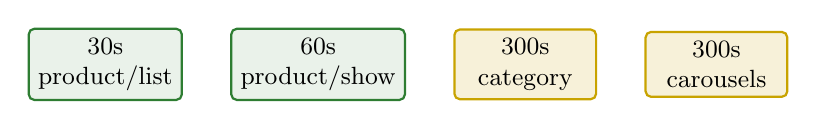
\begin{tikzpicture}[node distance=4mm and 6mm]
  \node[node-box,node-ok] (t1) {30s\\product/list};
  \node[node-box,right=of t1,node-ok] (t2) {60s\\product/show};
  \node[node-box,right=of t2,node-warn] (t3) {300s\\category};
  \node[node-box,right=of t3,node-warn] (t4) {300s\\carousels};
\end{tikzpicture}
\vspace{2mm}
\begin{itemize}
  \item \textbf{TTL = 业务可容忍的"用户看到老数据的最大时长"}。
  \item 列表 30s：翻页快照本来就有损，30s 足够。
  \item 详情 60s：调价后 1 分钟同步全网，运营接受。
  \item 分类 / 轮播 300s：天级变动 + 留余量做灰度发布。
  \item \textbf{TTL 越长越省钱，越短越新鲜}，两个角度业务侧自己拉锯。
\end{itemize}
\srcnote{routes/router.go:39--44 四个 GET 的 TTL 选型}
\end{frame}

% ============================================================
\section{异步下单的业务承诺}
% ============================================================

\begin{frame}{同步下单：双 11 零点的真实链路}
\begin{tikzpicture}[node distance=4mm and 6mm,every node/.style={font=\scriptsize}]
  \node[node-box] (cli) {client};
  \node[node-box,right=of cli,node-ok] (res) {reserve\\Redis Lua};
  \node[node-box,right=of res,node-bad] (db) {INSERT order\\+ outbox};
  \node[node-box,right=of db] (mq) {publish\\cancel delay};
  \node[node-box,right=of mq] (ret) {return};
  \draw[arrow] (cli) -- (res);
  \draw[arrow] (res) -- (db);
  \draw[arrow] (db)  -- (mq);
  \draw[arrow] (mq)  -- (ret);
  \node[font=\scriptsize,below=4mm of db] {瓶颈：磁盘 fsync + 事务锁};
\end{tikzpicture}
\vspace{3mm}
\begin{itemize}
  \item 平时：30--50ms 一笔，舒舒服服。
  \item 零点：5 秒 3 万笔 $\to$ INSERT 那一段 p99 飙到 1.4s。
  \item 网关 502 $\to$ 前端重试 $\to$ 雪崩。
  \item Redis Lua 那段（reserve）顶得住 5w QPS，是 DB 那段顶不住。
\end{itemize}
\srcnote{service/order\_async.go:118--172 异步路径与同步路径对比}
\end{frame}

\begin{frame}{异步下单：把 DB 那段甩到后台}
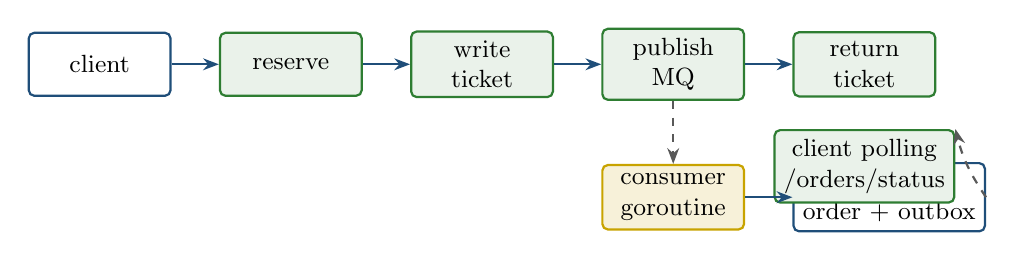
\begin{tikzpicture}[node distance=4mm and 6mm,every node/.style={font=\scriptsize}]
  \node[node-box] (cli) {client};
  \node[node-box,right=of cli,node-ok] (res) {reserve};
  \node[node-box,right=of res,node-ok] (tk)  {write\\ticket};
  \node[node-box,right=of tk,node-ok] (pub) {publish\\MQ};
  \node[node-box,right=of pub,node-ok] (ret) {return\\ticket};
  \node[node-box,below=8mm of pub,node-warn] (cons) {consumer\\goroutine};
  \node[node-box,right=of cons] (db) {INSERT\\order + outbox};
  \node[node-box,below=of ret,node-ok] (poll) {client polling\\/orders/status};
  \draw[arrow] (cli) -- (res);
  \draw[arrow] (res) -- (tk);
  \draw[arrow] (tk)  -- (pub);
  \draw[arrow] (pub) -- (ret);
  \draw[arrow-async] (pub.south) -- (cons.north);
  \draw[arrow] (cons) -- (db);
  \draw[arrow-async] (db.east) to[bend left=10] (poll.north east);
\end{tikzpicture}
\vspace{2mm}
\begin{itemize}
  \item 同步段只剩：reserve + 写 ticket + publish $\to$ < 10ms。
  \item DB 那段交给 consumer，prefetch=32 自然限速。
  \item 前端用 ticket 轮询 \texttt{/orders/status} 拿结果。
\end{itemize}
\srcnote{repository/rabbitmq/order\_async.go:50--71 ConsumeOrderAsync + Qos(32)；service/order\_consumer.go:51--102 落 DB}
\end{frame}

\begin{frame}{业务侧的"已受理"概念}
\begin{itemize}
  \item 异步化之后，HTTP 200 不再意味着"订单已落库"。
  \item 它的语义变成：\textbf{下单意图已被系统接受 + 库存已预占}。
  \item 这两件事就够了：用户不会被超卖、不会被重复扣款。
  \item DB 落库是\textbf{最终一致}的，秒级延迟用户感知不到。
\end{itemize}
\keypoint{业务承诺从"已下单"降级到"已受理"——但用户感知反而更好（不转圈）。}
\srcnote{service/order\_async.go:23--29 OrderTicketStatus 三态 pending/ok/failed}
\end{frame}

\begin{frame}{两条链路的用户感知时间线}
\begin{tikzpicture}[every node/.style={font=\scriptsize,align=center}]
  % 同步线
  \draw[arrow,draw=cBad,thick] (0,2) -- (12,2);
  \node[above=1mm] at (0,2)  {0ms};
  \node[above=1mm] at (12,2) {1.4s p99 / 5s 超时};
  \node[below=1mm,fill=cBad!15,rounded corners=2pt,inner sep=2pt] at (5,2) {同步：等转圈};
  \node[left=2mm of {(0,2)}] {同步};

  % 异步线
  \draw[arrow,draw=cOK,thick] (0,0) -- (12,0);
  \node[above=1mm] at (0,0)  {0ms};
  \node[above=1mm] at (1.5,0) {<10ms 拿 ticket};
  \node[above=1mm] at (4.5,0) {500ms 轮询};
  \node[above=1mm] at (7.5,0) {1s / 2s / 3s};
  \node[above=1mm] at (10.5,0) {3s+ 改长等待};
  \node[below=1mm,fill=cOK!15,rounded corners=2pt,inner sep=2pt] at (1.5,0)  {下单中};
  \node[below=1mm,fill=cOK!15,rounded corners=2pt,inner sep=2pt] at (6,0)    {spinner};
  \node[below=1mm,fill=cWarn!15,rounded corners=2pt,inner sep=2pt,align=center] at (10.5,0) {系统繁忙\\查订单列表};
  \node[left=2mm of {(0,0)}] {异步};
\end{tikzpicture}
\vspace{3mm}
\begin{itemize}
  \item 用户其实不在乎"几毫秒"，在乎\textbf{有没有反馈}。
  \item 异步链路一上来就给 ticket，前端可以\textbf{立刻}显示"下单中"。
  \item 超过 3 秒切"长等待"文案 + 一键去订单列表，转化损失最小化。
\end{itemize}
\srcnote{docs/blog/07-order-async-buffer.md 轮询节奏建议 500ms / 1s / 2s / 3s}
\end{frame}

\begin{frame}{ticket 过期 / 丢失的兜底}
\begin{itemize}
  \item Redis ticket TTL = \textbf{1 小时}（service/order\_async.go:24）。
  \item 用户拿到 ticket 就关了浏览器：consumer 落 DB 成功 $\to$ ticket 写 ok $\to$ 静静躺在 Redis 1 小时。
  \item 用户 30 分钟后回来：\textbf{ticket 还在}，能查到订单号；或者直接去订单列表能看见。
  \item TTL 到期 + 用户找客服："我下了单但没拿到订单号"：
  \begin{itemize}
    \item 客服按 \textbf{idempotency-key + userID + 时间窗}反查 order 表。
    \item idempotency 中间件保证同 key 只下一单（业务码 60002），可以追溯。
  \end{itemize}
\end{itemize}
\srcnote{service/order\_async.go:24 OrderTicketTTL = time.Hour；routes/router.go:80 enqueue 也挂 Idempotency}
\end{frame}

% ============================================================
\section{压测数字对照}
% ============================================================

\begin{frame}{基线 vs 两个升级（实测 + 推算）}
\begin{tabular}{@{}lrrr@{}}
\toprule
链路 & RPS & p95 & 来源 \\
\midrule
ping 基线              & 64{,}254 & 3.51ms & 实测 \\
商品详情（不挂 cache） & 62{,}226 & 3.01ms & 实测 \\
商品详情（304 命中）   & $\approx$ ping 基线 & <1ms & 推算 \\
\midrule
同步 /orders/create   & 50{,}319 & 2.33ms & 实测 \\
异步 /orders/enqueue  & $\approx$ ping 基线 & <10ms & 推算 \\
\bottomrule
\end{tabular}
\vspace{2mm}
\begin{itemize}
  \item ETag 304 不写 body，理论 RPS 逼近裸 gin 基线。
  \item enqueue 的同步段只剩 reserve + 写 Redis + publish，RTT 量级 ms。
  \item \textbf{两者都把瓶颈从"业务逻辑"挪到了"网络 + 中间件链"}，DB 不再是上限。
\end{itemize}
\srcnote{stressTest/REPORT.md \S 各链路压测表 1--7 行}
\end{frame}

\begin{frame}{接口 SLO 的前后对照}
\begin{tabular}{@{}llll@{}}
\toprule
接口 & 原 p95 & 优化后 p95 & 业务承诺 \\
\midrule
product/show   & 3.01ms & <1ms (304)   & 首屏快 + 带宽省 \\
product/list   & ms 级  & <1ms (304)   & 翻列表丝滑 \\
orders/create  & 2--50ms & <10ms (enqueue) & 零点不丢单 \\
\bottomrule
\end{tabular}
\vspace{3mm}
\small 对照 deck 10 的 SLO 表：P0 (orders/create) 承诺 99.95\% / p99 < 500ms。\\
异步化后 p99 从"DB 不可控"变成"MQ + Redis 可控"，error budget 烧得慢得多。
\srcnote{stressTest/REPORT.md \S 链路压测表；docs/slides/10-business-traffic-governance.tex SLO 表}
\end{frame}

\begin{frame}{两个升级各自的回滚预案}
\begin{tabular}{@{}lll@{}}
\toprule
升级 & 故障形态 & 回滚动作 \\
\midrule
HTTP cache & 用户看到老价格客诉 & TTL 改 0，只走协商缓存 \\
HTTP cache & 304 比对耗 CPU     & 整条 middleware 摘掉 \\
异步下单   & consumer 挂        & 监控积压告警 + 切回同步 \\
异步下单   & ticket 永久 pending & TTL 1h 自然清理 + 客服反查 \\
\bottomrule
\end{tabular}
\vspace{2mm}
\begin{itemize}
  \item HTTP cache 摘除是\textbf{单行 router 改动}，秒级回滚。
  \item 异步下单切回是\textbf{前端按钮切流量}，新接口 enqueue 失败时已经 fallback 同步 create。
  \item 两者都\textbf{不破坏旧接口语义}，回滚不需要数据迁移。
\end{itemize}
\srcnote{routes/router.go:39--44, 78--81 新旧接口共存}
\end{frame}

\begin{frame}{静默降级的代码模式}
\begin{tikzpicture}[node distance=8mm and 12mm]
  \node[node-state,node-state-normal] (a) {RMQ\\available};
  \node[node-state,node-state-alert,right=of a] (b) {RMQ\\unavailable};
  \node[node-box,right=of b] (rec) {recover\\warn log};
  \node[node-box,below=of b,node-ok] (sync) {同步 create\\不受影响};
  \draw[arrow] (a) -- node[above,font=\tiny]{init panic} (b);
  \draw[arrow] (b) -- (rec);
  \draw[arrow-alert] (b) -- (sync);
\end{tikzpicture}
\vspace{2mm}
\begin{itemize}
  \item \texttt{tryInitRabbitMQ} 用 \texttt{defer recover} 套住 panic，warn 日志后继续。
  \item Consumer 没起来：\texttt{/orders/enqueue} publish 阶段报错，前端 fallback 同步 \texttt{/orders/create}。
  \item ES / Web3 / Milvus 用同一套路 $\to$ \textbf{基础设施挂一个不连坐}。
\end{itemize}
\srcnote{cmd/main.go:54--62 tryInitRabbitMQ; :64--73 tryInitES; :86--97 tryInitMilvus}
\end{frame}

\begin{frame}{产品 / 运营 / 客服 / SRE 关心什么}
\begin{tabular}{@{}llll@{}}
\toprule
角色 & 关心 & HTTP cache 看 & 异步下单看 \\
\midrule
产品 & 转化率   & 首屏 LCP        & ticket 落单成功率 \\
运营 & 大促节奏 & CDN 命中率      & enqueue p95 \\
客服 & 投诉单   & "显示老价格"    & "下单中无响应" \\
SRE & 容量    & DB / ES 回源 QPS & consumer 积压 \\
\bottomrule
\end{tabular}
\vspace{3mm}
\small 四个角色看同一个升级的不同切面：\\
产品看的是收益，运营 / SRE 看的是水位，客服看的是异常。\\
任何一个面"看不见" $\to$ 这个升级就缺一只眼睛。
\srcnote{对照 deck 10 的"各角色关心的指标 + error budget"}
\end{frame}

\begin{frame}{运营关心：CDN 命中率怎么监控}
\begin{itemize}
  \item gomall 自身不接 CDN（单机部署），但 ETag 收益直接体现在：
  \begin{itemize}
    \item \textbf{后端 304 比例}：访问日志 status=304 占 GET 总数。
    \item \textbf{出网带宽}：商品域同时段 Gbps，预期降 60--80\%。
    \item \textbf{Redis / DB 读 QPS}：商品域 read replica 应当掉一个数量级。
  \end{itemize}
  \item 大促前一周抓 baseline，大促当天看曲线。
  \item 命中率<50\% $\to$ 检查前端是否丢了 If-None-Match 头 / TTL 是否过短。
\end{itemize}
\srcnote{middleware/httpcache.go:81--88 304 响应路径，可由 access log 区分}
\end{frame}

\begin{frame}{SRE 关心：consumer 积压告警怎么设}
\begin{itemize}
  \item RMQ 队列 \texttt{order.create.async.queue} 深度 = \textbf{核心 SLI}。
  \item 三档告警：
  \begin{itemize}
    \item P3：深度 > 1000 持续 1min $\to$ 钉钉提醒
    \item P1：深度 > 10000 持续 30s $\to$ 电话值班
    \item P0：深度 > 100000 或 consumer 全停 $\to$ 自动切回同步路径
  \end{itemize}
  \item 自动切回的开关：网关侧把 \texttt{/orders/enqueue} 流量改路由到 \texttt{/orders/create}。
  \item 这意味着前端拿到的不再是 ticket 而是订单号，UI 侧需要兼容两种响应。
\end{itemize}
\srcnote{repository/rabbitmq/order\_async.go:11--15 队列名 OrderAsyncQueue}
\end{frame}

% ============================================================
\section{回到业务：性能即业务}
% ============================================================

\begin{frame}{把这一份 deck 浓缩成一句话}
\begin{itemize}
  \item HTTP cache 不是"加层缓存"，是\textbf{让浏览器替后端挡 80\% 流量}。
  \item 异步下单不是"换 MQ"，是\textbf{把"用户等"换成"系统排队"}。
  \item 两者都不动业务语义，都\textbf{加在已有接口的旁边}，挂了能秒切回。
  \item 业务方拿到的是两条具体承诺：\textbf{运营推爆款不打挂详情、双 11 零点不丢单}。
\end{itemize}
\keypoint{性能升级的衡量标准不是"快了多少毫秒"，是"挽救了多少 GMV、省了多少带宽、少接了多少客诉"。}
\end{frame}

% ============================================================
\appendix
% ============================================================

\begin{frame}{业务 Q\&A（上）}
\textbf{Q1}：ETag vs Last-Modified vs Cache-Control，业务侧怎么选？\\
\hspace{4mm}\small A：\texttt{Cache-Control: max-age} 是\textbf{强缓存}，TTL 内根本不发请求，省 RTT。
\texttt{ETag / Last-Modified} 是\textbf{协商缓存}，仍发请求但服务端可以 304 省 body。
Last-Modified 精度到秒，对秒级变更（商品改价）会误判；ETag 走 body 摘要，精确。
gomall 选 Cache-Control + ETag 双管齐下：60s 内零请求，过期发协商。

\vspace{2mm}
\textbf{Q2}：cache 击穿时的 SETNX 回源锁怎么和 ETag 配合？\\
\hspace{4mm}\small A：两者治理的是不同层。SETNX 锁挡的是\textbf{服务端 Redis 失效后多并发回源 DB}；
ETag 挡的是\textbf{客户端层重复请求}。一个用户 If-None-Match 命中 304 $\to$ 根本不进 Redis 那一层 $\to$ 也不会触发回源锁。两个机制独立工作，互不影响。

\vspace{2mm}
\textbf{Q3}：ticket TTL 1h，用户 2 小时后回来怎么办？\\
\hspace{4mm}\small A：ticket 没了，但订单大概率已经在 \texttt{orders/list} 里。
极端场景（consumer 失败 + ticket 过期）：客服按 idempotency-key + userID + 时间窗反查。
TTL 选 1h 是平衡 Redis 内存（千万级 ticket = GB 级）与"用户回看耐心"的结果。
\end{frame}

\begin{frame}{业务 Q\&A（下）}
\textbf{Q4}：异步下单跟秒杀场景怎么合纳？\\
\hspace{4mm}\small A：秒杀走 \texttt{/skill\_product/skill}，挂滑动窗口 3/s/用户，主要拦黑产。
普通双 11 / 限时活动走 \texttt{/orders/enqueue}，主要削 DB 峰。
两者可以叠加：秒杀通过后转 enqueue 落库，DB 完全不见瞬时峰。

\vspace{2mm}
\textbf{Q5}：双 11 之外平时是否启用异步？\\
\hspace{4mm}\small A：可以。平时 \texttt{/orders/enqueue} p95 < 10ms，比同步 30--50ms 还快。
但有两个代价：(a) 前端要多写一段轮询；(b) ticket 给运维多一类需要监控的对象。
小公司建议平时同步、大促异步，前端按 feature flag 切。

\vspace{2mm}
\textbf{Q6}：CDN 命中率怎么监控？\\
\hspace{4mm}\small A：(a) 后端访问日志按 status=304 分组，看 304 / (200+304) 比例；
(b) 接 CDN 厂商的话直接看 CDN 控制台命中率；
(c) 看 DB / ES read QPS 变化幅度，副指标但很可靠。
gomall 单机部署只能用 (a) + (c)。
\end{frame}

\begin{frame}{代码位置一览}
\begin{description}
  \item[HTTP cache 中间件]\srcnote{middleware/httpcache.go:47--100}
  \item[弱 ETag 算法]\srcnote{middleware/httpcache.go:103--106 SHA-256 前 16 字节}
  \item[公开 GET 挂载点]\srcnote{routes/router.go:39--44 product/list, product/show, category, carousels}
  \item[异步下单入口]\srcnote{routes/router.go:80 /orders/enqueue + Idempotency}
  \item[ticket 状态查询]\srcnote{routes/router.go:81 /orders/status}
  \item[OrderEnqueue 主流程]\srcnote{service/order\_async.go:119--172}
  \item[ticket 三态定义]\srcnote{service/order\_async.go:23--29}
  \item[consumer 落 DB + outbox]\srcnote{service/order\_consumer.go:51--102}
  \item[RMQ 拓扑]\srcnote{repository/rabbitmq/order\_async.go:11--32}
  \item[publish / consume]\srcnote{repository/rabbitmq/order\_async.go:35--72}
  \item[消费者启动 + 静默降级]\srcnote{initialize/order\_async.go:13--29}
  \item[main 静默降级套路]\srcnote{cmd/main.go:54--97 四个 tryInit*}
\end{description}
\vspace{2mm}
\keypoint{配套博客：docs/blog/06-http-cache.md \& docs/blog/07-order-async-buffer.md}
\end{frame}

\end{document}
